
%\RequirePackage{pdf15}

\documentclass{beamer}

\usepackage[utf8]{inputenc}

\usepackage{mystyle}

\usepackage{natbib}
\usepackage{tikz}
\usepackage{pgfplots}

%Information to be included in the title page:
\title{Scaling Hidden Markov Language Models}
\author{Anonymous}
\date{2020}



\begin{document}

\frame{\titlepage}

\begin{frame}
\frametitle{Motivation for HMMs}
\begin{itemize}
\item Generative process separates the generation of the latent representations from the observed
    \begin{itemize}
    \item LSTMs couple the two
    \end{itemize}
\item Discrete latent representations
    \begin{itemize}
    \item Improves performance in low-resource classification (citation todo)
    \end{itemize}
\end{itemize}
\end{frame}

\begin{frame}
\frametitle{HMM LMs}
\begin{itemize}
\item Previously thought to be very poor language models 
    \begin{itemize}
    \item Improved performance by departing from HMM structure and turning them into RNNs \citep{buys2018hmm}
    \end{itemize}
\item HMMs performance can be vastly improved by scaling the number of hidden states
\end{itemize}
\end{frame}

\begin{frame}
\frametitle{HMMs}

\begin{center}
\begin{tikzpicture}[]
\node[latent] (z0) {$z_0$} ;
\node[latent] (z1) [right=1.25cm of z0] {$z_1$} ;
\node[latent] (z2) [right=1.25cm of z1] {$z_2$} ;
%\node (dots) [right=1.25cm of z2] {$\cdots$} ;
%\node[latent] (zt) [right=1.25cm of dots] {$z_T$} ;

\node[obs]    (x0) [below = 0.75cm of z0] {$x_0$};
\node[obs]    (x1) [below = 0.75cm of z1] {$x_1$};
\node[obs]    (x2) [below = 0.75cm of z2] {$x_2$};
%\node (adots) [right=1.25cm of x2] {$$} ;
%\node[latent] (xt) [right=1.25cm of adots] {$x_T$} ;

\edge {z0} {x0};
\edge {z1} {x1};
\edge {z2} {x2};
\edge {z0} {z1};
\edge {z1} {z2};
%\edge {z2} {zt};
%\edge {dots} {zt};

\end{tikzpicture}
\end{center}


Joint distribution
\begin{equation*}
p(\bx, \bz; \theta)
= \prod_{t=1}^T p(x_t\mid z_t)p(z_t \mid z_{t-1})
\end{equation*}
We shorten the emission matrix $p(x_t \mid z_t)$ to $\mathbf{O}$.
\end{frame}

\begin{frame}
\frametitle{Training HMMs}
\begin{itemize}
\item Computing the likelihood of the observed sentence is $O(T|\mcZ|^2)$,
    scaling poorly in the number of states
\item Tabular parameterizations of distributions are difficult to optimize
\item We present three tricks to mitigate these issues
\end{itemize}
\end{frame}

\begin{frame}
\frametitle{3 Tricks 4 Scaling HMMs}
\begin{itemize}
\item A block-sparse emission matrix reduces the computational cost of computing the likelihood
\item A compact (neural) parameterization of the transitions and emissions
    aides optimization
\item State dropout further reduces computational cost and reduces overfitting
\end{itemize}
\end{frame}

\begin{frame}
\frametitle{Block-sparse Emissions}
\begin{itemize}
\item Constrain emissions to
\[\mathbf{O} = \begin{bmatrix} \mathbf{O}^1 & 0 & 0 \\ 0 & $\dots$ & 0 \\ 0 & 0 & \mathbf{O}^M \\
\end{bmatrix}\]
\item Each block $\mathbf{O}_m$ contains $k$ latent states and a variable number of tokens
\item Results in a serial complexity of $O(Tk^2)$ for computing the likelihood
\end{itemize}
\end{frame}

\begin{frame}
\frametitle{Block-sparse Emissions}
\centering
\input{img/trellis_nodrop.tex}
\end{frame}

\begin{frame}
\frametitle{Neural Parameterization}

\begin{itemize}
\item Compute transition and emission parameters using a neural network
\begin{itemize}
\item State embeddings $\mathbf{E}_z \in \mathbb{R}^{|\mcZ| \times h/2}$
\item Token embeddings $\mathbf{E}_x \in \mathbb{R}^{|\mcX| \times h}$
\item Block embeddings $\mathbf{E}_m \in \mathbb{R}^{M \times h/2}$
\end{itemize}
\end{itemize}

\vspace{0.5em}

\centering
\includegraphics[height=1.7in]{img/mat.png}

\end{frame}


\begin{frame}
\frametitle{State Dropout}
\begin{itemize}
\item Sample a dropout mask $\mathbf{b}_m \in \set{0,1}^k$ for each block $\mathbf{O}_m$
\item Concatenate into a global vector $\mathbf{b} = \langle \mathbf{b}_1, \ldots, \mathbf{b}_M \rangle$
\end{itemize}

\vspace{1em}
\centering
\resizebox{2in}{2in}{
\input{img/trellis.tex}
}
\end{frame}

\begin{frame}
\frametitle{Results on PTB}

\begin{table}[!t]
\centering
\begin{tabular}{llrr}
\toprule
Model & \# Params & Val PPL  & Test PPL\\
\midrule
KN 5-gram   & 2M & - & 141.2\\
AWD-LSTM  & 24M & 60.0 & 57.3\\
256 FF 5-gram  & 2.9M     & 159.9      & 152.0  \\
2x256 dim LSTM  & 3.6M     & 93.6       & 88.8   \\
HMM+RNN   & 10M & 142.3 & -\\
HMM ($|\mcZ|$=900) & 10M & 284.6 & -\\
VL-NHMM ($|\mcZ|=2^{15}$)   & 7.7M     & 125.0      & 115.8  \\
\bottomrule
\end{tabular}
\end{table}

\end{frame}

\begin{frame}
\frametitle{Results on WikiText2}

\begin{table}[!t]
\centering
\begin{tabular}{llrr}
\toprule
Model & \# Param & Val PPL & Test PPL\\
\midrule
KN 5-gram & 5.7M       & 248.7 & 234.3\\
AWD-LSTM & 33M & 68.6 & 65.8\\
256 FF 5-gram        & 8.8M    & 210.9  & 195.0\\
2x256  LSTM     & 9.6M    & 124.5  & 117.5\\
%32k state HMM (no fac)   & 17.3M   & 166.7  & -\\
VL-NHMM ($|\mcZ|=2^{15}$)           & 13.7M   & 169.0      & 158.2\\
\bottomrule
\end{tabular}
\end{table}

\end{frame}

\begin{frame}
\frametitle{State Size Ablation}

\centering
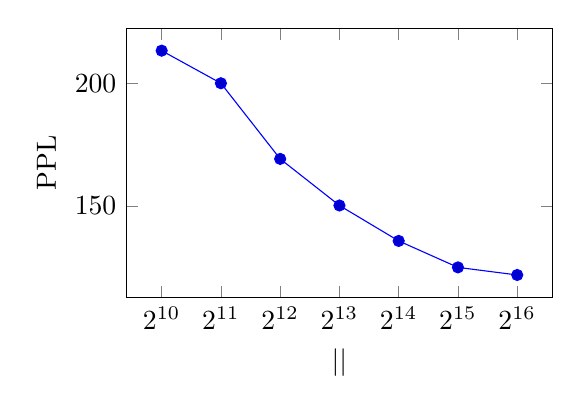
\begin{tikzpicture}
\begin{axis}[
    xlabel=$|\mcZ|$,
    ylabel=PPL,
    xmode=log,
    log basis x={2},
    xtick={},
    width=7cm,
    height=5cm
]
\addplot plot coordinates {
(1024,  213.25)
(2048,  199.98)
(4096,  169.18)
(8192,  150.22)
(16384, 135.79)
(32768, 125.02)
(65536, 121.93)
};
\end{axis}
\end{tikzpicture}

Perplexity on PTB by state size $|\mcZ|$ ($\lambda =0.5$ and $M=128$)
\end{frame}

\begin{frame}
\frametitle{Bibliography}
\bibliographystyle{acl_natbib}
\bibliography{anthology,emnlp2020}
\end{frame}

\end{document}
